%! Author = mackesmilian
%! Date = 01.11.21

% Preamble
\documentclass[11pt]{article}
\usepackage{graphicx}
\usepackage{xr}
\usepackage[english]{babel}
\usepackage[style=apa]{biblatex}
\usepackage{float}
\addbibresource{main.bib}
\usepackage{csquotes}
\graphicspath{ {/home/mackesmilian/Documents/FH/BACC/bachelorarbeit/src/images/} }
\title{
        {Development and Deployment of Web Applications as Installable Desktop Applications Using
    Electron Framework}\\
    {\large FH Campus 02}\\
}
\author{Maximilian Martin Wolf}
\date{30 October 2021}
% Document
\begin{document}

    \maketitle
    \pagebreak
    \tableofcontents
    \pagebreak


    \section{Introduction}\label{sec:introduction}
    \setcounter{tocdepth}{3}

    \subsection{What Is Electron?}\label{subsec:what-is-electron}
    In December 2012 software engineer Cheng Zhao joined GitHub's team, having previously worked for Intel developing
node-webkit, with the task of porting the Atom editor from using Chromium Embedded Framework to node-webkit.
Node-webkit being a Node.js module developed by Roger Wang which combined the browser engine used by Chromium - WebKit - 
with Node.js, making Node.js modules accessible from JavaScript code running inside a web page. \parencite{jensen2017}\paragraph{}

Porting to node-webkit proved difficult, so GitHub abandoned that approach, and it was decided that a new native shell
for Atom would be created.
Said shell was dubbed \emph{Atom Shell} and after development was finished and the Atom editor was open sourced
by GitHub, Atom Shell soon followed suit and was renamed to \emph{Electron}.
Initially developed as a way to deliver an editor, numerous widely known applications like Slack, Discord and Visual
Studio have started using Electron to develop and deliver their desktop applications.\parencite{electronDocs}
But what exactly is Electron?\paragraph{}
Electron is a framework which allows for the development of cross-platform desktop applications using only popular 
web programming languages like HTML, CSS and JavaScript. 
While the advantages will be discussed in detail in the next chapter \emph{Why Use Electron?}, the appeal to developers
is obvious: Maintaining one codebase while being able to deliver the app to all desktop operating systems.\paragraph{}
Now, as described previously the Electron framework serves the same purpose as node-webkit (later renamed to NW.js), but
their approaches do differ in certain ways: \parencite{jensen2017}\par
\begin{figure}[ht]
    \label{fig:el-architecture}
    \caption{A simplified representation of Electron's architecture. \parencite{jensen2017}}
    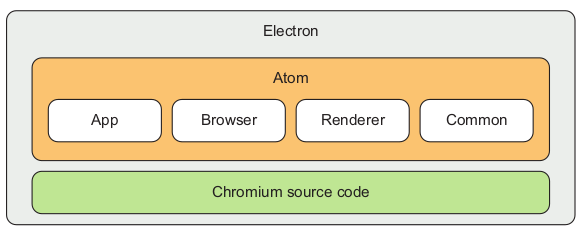
\includegraphics[width=\textwidth]{electron-architecture}
\end{figure}
Without going into detail on how NW.js works, Electron and NW.js share some architectural similarities.
However, there are some differences in how Electron combines Node.js with Chromium.\paragraph{}
Architecturally, Electron places an emphasis on strict separation from Chromium source code, ass seen in figure \ref{fig:el-architecture}.
This looser integration allows for easier updates to the Chromium part of the source code, whereas with NW.js Chromium
is patched to allow for Node.js and Chromium to use a shared Javascript state. \parencite{jensen2017}\par
On the other hand, this means that Electron has separate JavaScript contexts: A \emph{main} process which starts running
with the app window and a \emph{renderer} process for each individual window.
Any sharing of state between these contexts, or simply put between the front- and back-end, has to pass through the
\emph{icpMain} and \emph{icpRenderer} modules.
This means that each JavaScript context is kept separate but data can be explicitly shared, allowing for greater control
over what state exists in which app window. \parencite{jensen2017}\paragraph{}
Electron itself (the part without Chromium) is made up of for different components: App, Browser, Renderer and Common.
\textbf{App} contains code written in C++ and Objective-C++ responsible for loading Node.js and Chromium's content module.
The \textbf{browser} folder contains code which handles interactions with the front-end.
This is to say functionality such as loading the JavaScript engine, interacting with the UI and binding operating system
specific modules.
As for \textbf{renderer}, this component handles the different renderer processes.
Because Chromium works by running each tab as an individual process, as to not crash the entire browser should one
tab become unresponsive, each application window in Electron runs as its own process.
\textbf{Common} contains code which is used by both the main and renderer processes for running the application.
Among other things this folder also contains the integration of Node.js' event loop with Chromium's event loop. \parencite{jensen2017}\paragraph{}


    \subsection{Why Use Electron?}\label{subsec:why-use-electron}
    Now the next obvious question is why a framework such as Electron is needed at all.
After all, it is "just" a way to have desktop applications developed using HTML, CSS and JavaScript.
So why not just develop native desktop applications or traditional web applications depending on the use case?
To answer this one has to examine the bigger picture:\paragraph{}
Over the past decade it seems as though software pricing has moved from perpetual licenses towards subscription-based
models.
If one examines the data regarding end-user spending on cloud applications it is clear that the
\emph{Software as a Service} (SaaS) model has grown considerably in revenue and is projected to do so in the future:
The worldwide end user spending for Software as a Service has increased from 31.4 billion US Dollars in 2015 to 120
billion US Dollars in 2020.
It is projected this growth will progress with spending reaching 171.9 billion dollars in 2022. \parencite{gartner2021}\paragraph{}
Furthermore, \textcite{gartner2021} forecasts that by 2026, cloud spending will exceed 45\% of all enterprise IT spending, up from
17\% in 2021.
This impressive growth can be attributed to two reasons.
Reasons either technical and/or financial in nature.
One financial benefit of SaaS is economies of scale:
By hosting the application centrally and by extension aggregating users together, providers can benefit financially from
leveraging economies of scale.
At the simple end, this means benefiting from volume pricing on hardware such as data centers, servers, space and so on.
Taking this idea further, SaaS providers can also cut costs by sharing hardware across their customers.
It is not cost-effective to use one machine for each customer, instead resources should be shared and dynamically
allocated on-demand to each customer's needs.
Similarly, as user count increases, the cost of adding on single user decreases.
These and other reasons are a big financial motivator for providers of software to switch to the SaaS model.\paragraph{}
However, technological reasons play a large role as well.
According to \textcite{jacobs2005} the ever-increasing maturity of the Web is a major contributor for the rise in popularity of
SaaS.\par
Browsers are significantly more powerful than ever. 
The \emph{browser wars} of the mid-to-late nineties started with Microsoft and Netscape outdoing each other with
new features, faster and overall better browsers leading to significant leaps in browser technology. \parencite{mozilla2021,jensen2017}\paragraph{}
Furthermore, internet access is more widespread than ever.
In the United States, the number of internet users rose from 229,91 million in 2010 to 302,28 million in 2021,
which constitutes a 31\% increase.\par
\begin{figure}[H]
    \centering
    \label{fig:num-of-internet-users}
    \caption{Number of internet users in the US from 2010 to 2025. \parencite{statista2021}}
    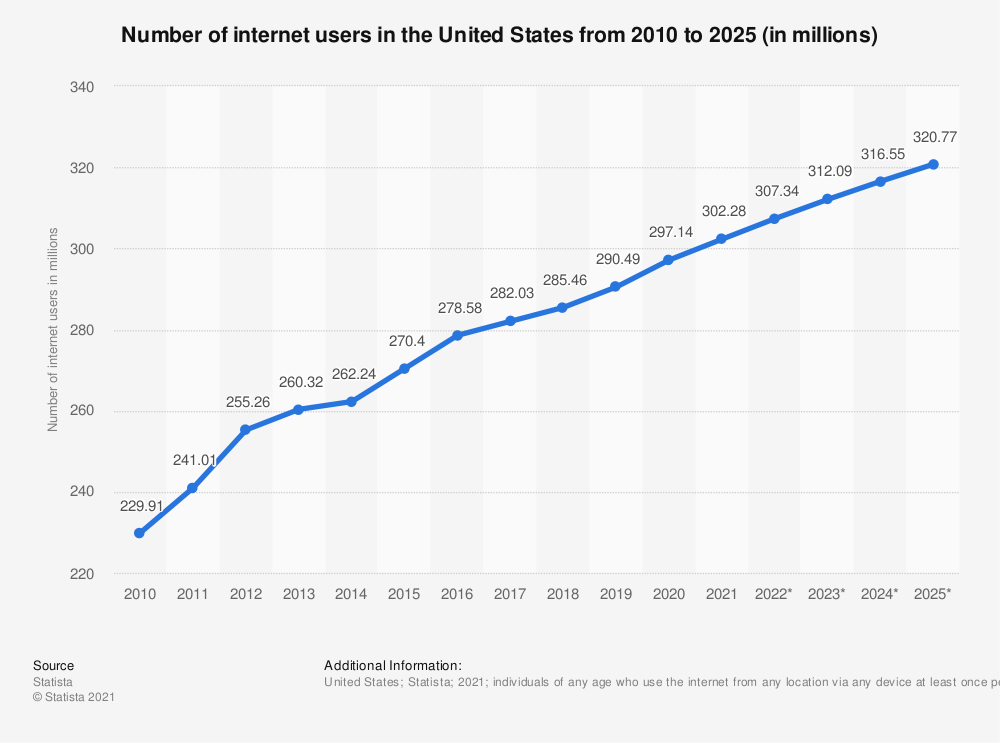
\includegraphics[width=0.8\textwidth]{number-of-internet-users}
\end{figure}
And not only have the number of internet users risen over the past eleven years, the average connection speed increased as well
over the same time period:
\begin{figure}[H]
    \centering
    \label{fig:internet-speed}
    \caption{Average internet connection speed in the US 2007-2017. \parencite{akamai2017}}
    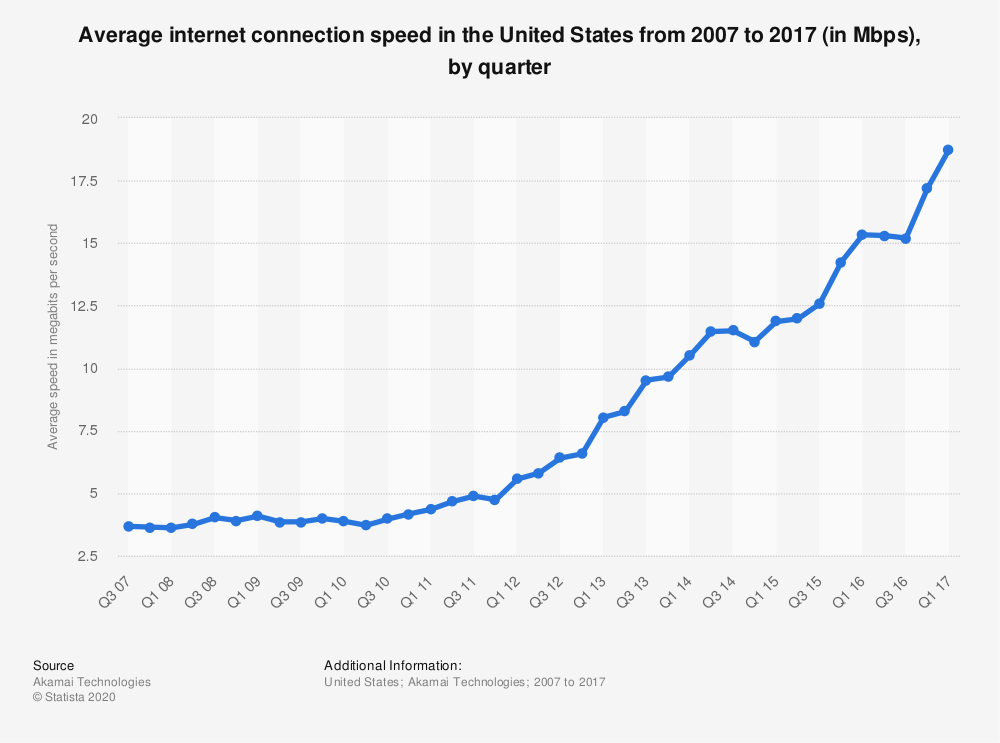
\includegraphics[width=0.8\textwidth]{internet-connection-speed}
\end{figure}
As seen above, from Q3 2017 to Q1 2017, average internet speeds across the US rose by 410\%.
This allowed for much more elaborate websites where larger amounts of data have to be downloaded.
Moreover, the number of robust frameworks for web development (be it front-end or back-end), make creating a complex web application easier
than ever before.
However, while this explains why SaaS is often the billing model of choice, it doesn't fully explain why specifically web applications
have risen in popularity. \parencite{statista2021}\par
After all, SaaS can also be delivered as a Desktop Application, as seen with the Adobe Creative Suite for example. \parencite{adobe2021}\par
To answer this, one should examine how desktop applications and web applications differ in more detail.



    \subsubsection{Desktop Applications}\label{subsubsec:desktop-applications}
    Desktop applications used to be the standard way of delivering software to the end user.
Users had to go to a store, buy a CD-ROM, check the system requirements and install the software 
on their machine.
This does of course come with a number of benefits over web applications.\par
One advantage is that desktop applications aren't reliant on an internet connection.
Web applications obviously fail here, as their are accessed over the internet.
Furthermore, this reliance on an internet connection leads to more issues when the application
is very feature-rich and/or has to support large files. 
An image editing software as a web application for example can run into limitations when being
used with high-resolution images. 
Similarly, desktop applications start instantly without having to download resources over the 
internet. 
In such cases, desktop applications have an edge over comparable web applications.\cite{jensen2017}\par
There of course also benefits to using desktop applications from a developer's perspective.
As a developer, one does not have to worry about users accessing their web applications over different web browsers 
as the choice of browser is at the user's discretion. 
This means not having to consider how different browser interpret CSS, for example. 
Another benefit is the fact of tighter integration with the user's OS.
Browser security limits the use of hardware and can lead to challenges for certain use cases.\cite{jensen2017}\par
Moreover, another benefit of having an installable desktop application is not having to continuously support all the necessary infrastructure.
There simply is no need to run servers, databases and such when the application is locally installed on each user's machine.\cite{jensen2017}


    \subsubsection{Web Applications}\label{subsubsec:web-applications}
    \externaldocument{main.tex}
In contrast to desktop applications, the relatively low barrier for entry thanks to the easy of learning
the basics of HTML, CSS and JavaScript in web development makes it much easier for developers to create complex web applications. 
With the amount of open source frameworks developers of web apps have a large selection of different solutions to fit
their specific use case.
Also, package managers like npm offer a large selection of readily available, well established packages for developers to use
and enhance their projects.\paragraph{}
Another big advantage of web applications is that they are platform-independent. 
A web application can be reached on any reasonably modern device which runs a web browser.
There is no need to create a separate version for all the operating system one wants to support and 
websites can also easily be accessed on mobile devices.\paragraph{}
As described in the previous chapter \ref{subsubsec:desktop-applications}, web applications need continuously running infrastructure such as
web servers and databases. 
While this constitutes a disadvantage, it also comes with a big benefit for developers, as they can strictly control which version 
a client uses.
Furthermore, the access to real-world data in said databases makes reproducing bugs much simpler. \parencite{jacobs2005}

    \subsubsection{Electron as a Solution}\label{subsubsec:electron-as-solution}
    \externaldocument{main.tex}
However, web applications do come with disadvantages. 
As described in \ref{subsubsec:desktop-applications} web apps have their shortcomings such as 
browser security preventing access to a user's file system or having no access as soon as the internet connection
fails.\paragraph{}
This is where frameworks such as Electron manage to strike the near-perfect balance between desktop application and web app.
For instance the drawback of not having access to a user's PC's file system does not apply to applications 
developed using Electron, as the npm module \emph{osenv} can for example retrieve the user's home folder among 
other environment settings. \parencite{osenv}\paragraph{}
Additionally, the disadvantage of having to consider different browsers (and versions thereof) are a non-issue
with electron because Electron uses Chromium as outlined in \ref{subsec:what-is-electron}. 
Furthermore, internet access is not a requirement with Electron which means applications can have some offline
functionality as opposed to web apps.\par
These are some features and advantages of Electron, though not an exhaustive list. \parencite{electronDocs}\paragraph{}
Ultimately, it is at the developer's discretion which form of software to use.
Native desktop applications, web applications or applications developed using frameworks such as Electron 
all have advantages and disadvantages and it is important to consider
which solution fits an application's and/or user's needs best.\paragraph{}
During the course of this bachelor thesis, Electron will be evaluated as a framework for developing desktop applications
by implementing an example project. 
The aforementioned considerations and points will be examined in development of said application and 
finally an evaluation will be made on how effective of an alternative to web applications Electron is 
and whether the biggest shortfalls of web applications can be eliminated or mitigated by 
using Electron.

    \section{Method}\label{sec:method}
    \externaldocument{main.tex}
Using the Design Science approach \parencite{VaishnaviVijayKuechler} an artifact will be developed using Electron.
Said artifact is a proof-of-concept application which will be used to gauge whether Electron would be an effective
solution in this specific and other different use cases. \paragraph{}
The application to be developed will be developed similarly to an already existing application.
Said application is a time keeping app developed by and used by Comm-Unity GmbH, a company specialising in e-government
software.
This web app is used by all employees to record the time worked based on factors such as customers, projects and other
internal, domain-specific aspects.\paragraph{}
The existing application is a web-only application developed using Vaadin 
(Vaadin is a server-side Java-only framework for web development)\parencite{vaadinDocs}.
By developing a similar application using Electron one can directly judge where the advantages and 
disadvantages of Electron lie. 

    \subsection{Artifact Outline}\label{subsubsec:dev-requirements}
    \externaldocument{main.tex}
As mentioned before the intention of the application is to facilitate efficient time keeping 
for employees of Comm-Unity EDV GmbH. 
As with any business-oriented time keeping program it is central to be able to book 
time worked on specific data points not only to be able to bill customers correctly but also to 
create a clearer picture of which project and/or customer require what amount of attention by 
employees.
In this specific proof-of-concept we will limit said data points to customers and projects.\paragraph{}
These can be easily extended customised depending on domain-specific requirements and needs but as far 
as this example goes, a generalised approach is sufficient and also required as to extrapolate results 
on other use cases.\paragraph{}
The below described requirements have been deducted from decades long experience within the company in question.
As a comparable application has been in use for 20 years, users of this tool and engineers who were involved
in designing the legacy application have an extensive knowledge of what improvements were required.
These improvements were then defined as new features and continuously re-evaluated throughout development.
These re-evaluation cycles used input from software engineers with extensive company specific knowledge and
experienced users.
Therefore the requirements for the artifact created and discussed within this thesis were adopted from the existing
application developed for Comm-Unity EDV GmbH.\paragraph{}
The application will be structured into four different views. 
The main view shows a list of entries which each represent a data point.
Said data point has a start and end time a project and customer are assigned to each entry. 
As the number of customers and projects increases over time it becomes increasingly difficult for 
employees to quickly find the correct values to attribute their entries to.
To make this easier to use users can create templates which limit the possible data points one can
choose.\paragraph{}
The second view is the so called template view which shows a list of the aforementioned templates.
Users can create, update and delete templates which each have a unique ID, a name and a list of projects 
and customers.\paragraph{}
The third view is an overview of customers, which can be created, updated and removed. 
Each customer is comprised of a name and an address.\paragraph{}
The fourth view is similar to the customers view but represents an overview of projects, which 
can also be created, updated and removed.
Each project contains a name and whether said project is active or not.\paragraph{}

    \externaldocument{main.tex}
The application can be split into three distinct parts from a technological/architectural point of view:
\begin{itemize}
  \item The back-end API used to fetch and save data.
  \item The front-end part using Angular\parencite{angularDocs}.
  \item The Electron part used to deploy the application and to offer offline functionality.
\end{itemize}
The back-end uses a MongoDB \parencite{mongoDocs} database to persist data. 
The decision to choose MongoDB was taken because of the use
case: A time keeping application needs to be highly flexible.
Entities such as projects and customers and the general company structure and therefore evolving requirements can change over time, 
possibly necessitating a different database structure. 
Due to MongoDB being a No-SQL database based on a JSON-like document structure, future changes regarding documents (which are analogous to tables 
in relational databases) require no changes to the database itself.
Such flexibility would greatly increase the future proofing of such an application.\paragraph{}
The back-end logic is developed in Python and uses the Flask framework \parencite{flaskDocs} for handling
requests from the front-end.
As mentioned previously for each entity (project, customer, template, and entry) there is business
logic to support create, update, and remove operations.\paragraph{}
The front-end uses Angular \parencite{angularDocs} and Angular Material \parencite{angularMaterialDocs}.
Angular was chosen as it is a very popular framework for single page applications and furthermore,
it makes it easy to develop re-usable UI components.
As for the components library, Angular Material was used because of its ease of use and well-known design, 
meaning users can easily adjust to the new user interface.
\begin{figure}[H]
  \centering
  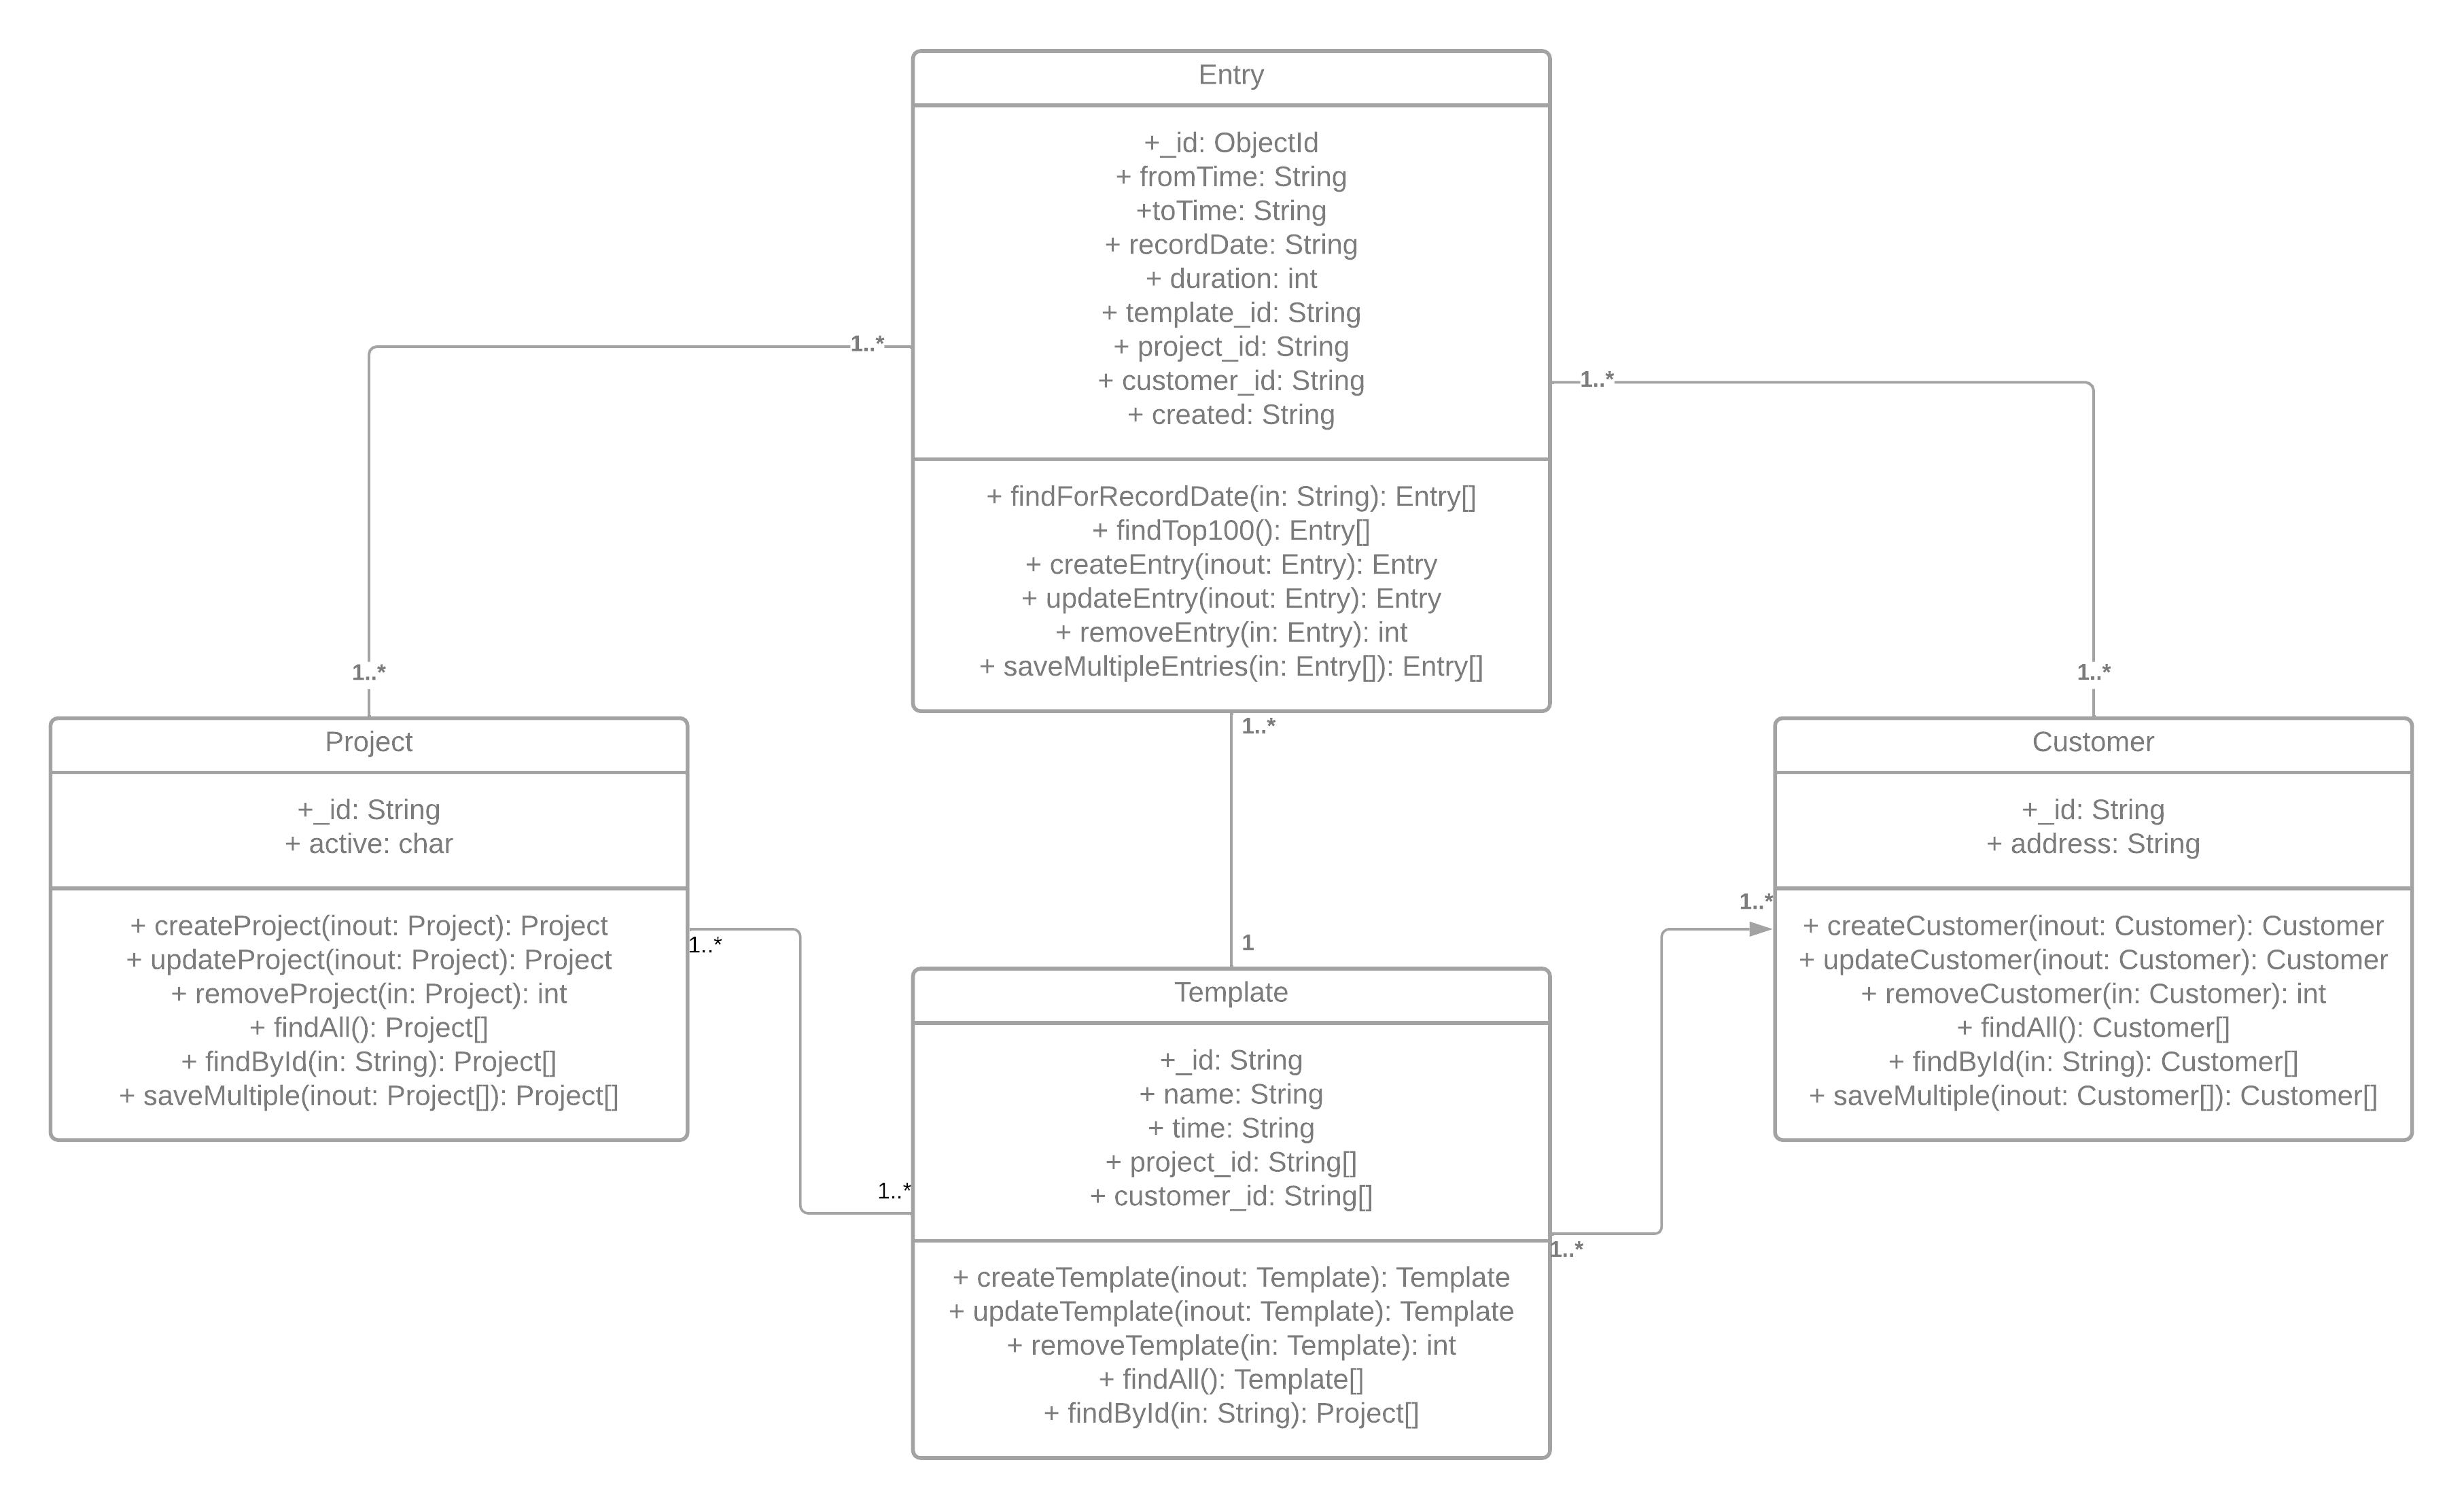
\includegraphics[width=1\textwidth]{pze-class-diagram}
  \caption{A class diagram representing all entities, relationships and operations.}
  \label{fig:pze-class-diagram}
\end{figure}
As seen in the figure above, all entities have similar operations and relationships. 
Each can be created, updated, and removed.
Furthermore, each offers an operation to fetch an entity based on its ID, as those are retrieved on-demand and not 
fetched eagerly.
Additionally, the Entry entity contains an operation to fetch the 100 latest entries (ordered by their recordDate attribute) in
order to return data for a local backup on each user's machine.
As the number of entries will grow once this is in use it is neither practical nor sensible to fetch all records from the database
just to make offline usage possible. 
Another unique operation of the Entry entity is fetching Entries based on their recordDate attribute. 
This is necessary as users view entries on a per-day basis.\paragraph{}
Entry, Project and Customer entities each contain an operation which allows for the creation of multiple of their respective entities.
This is to facilitate the offline functionality where users can create entities while not connected to the back-end API. 
Said entities are saved locally and once connection is restored, they are posted to the back-end and persisted.\paragraph{}
An instance of a template always references at least one customer and project, meaning that each entry which always references exactly one template 
always references at least one project and customer. 
One template can of course be referenced by multiple entries and one template can reference multiple project and vice-versa.
On the database level, a template holds an array of project and customer IDs as references.
The IDs of customer and project entities are a string representation of their given name as those have to be unique.\paragraph{}
\begin{figure}[H]
  \centering
  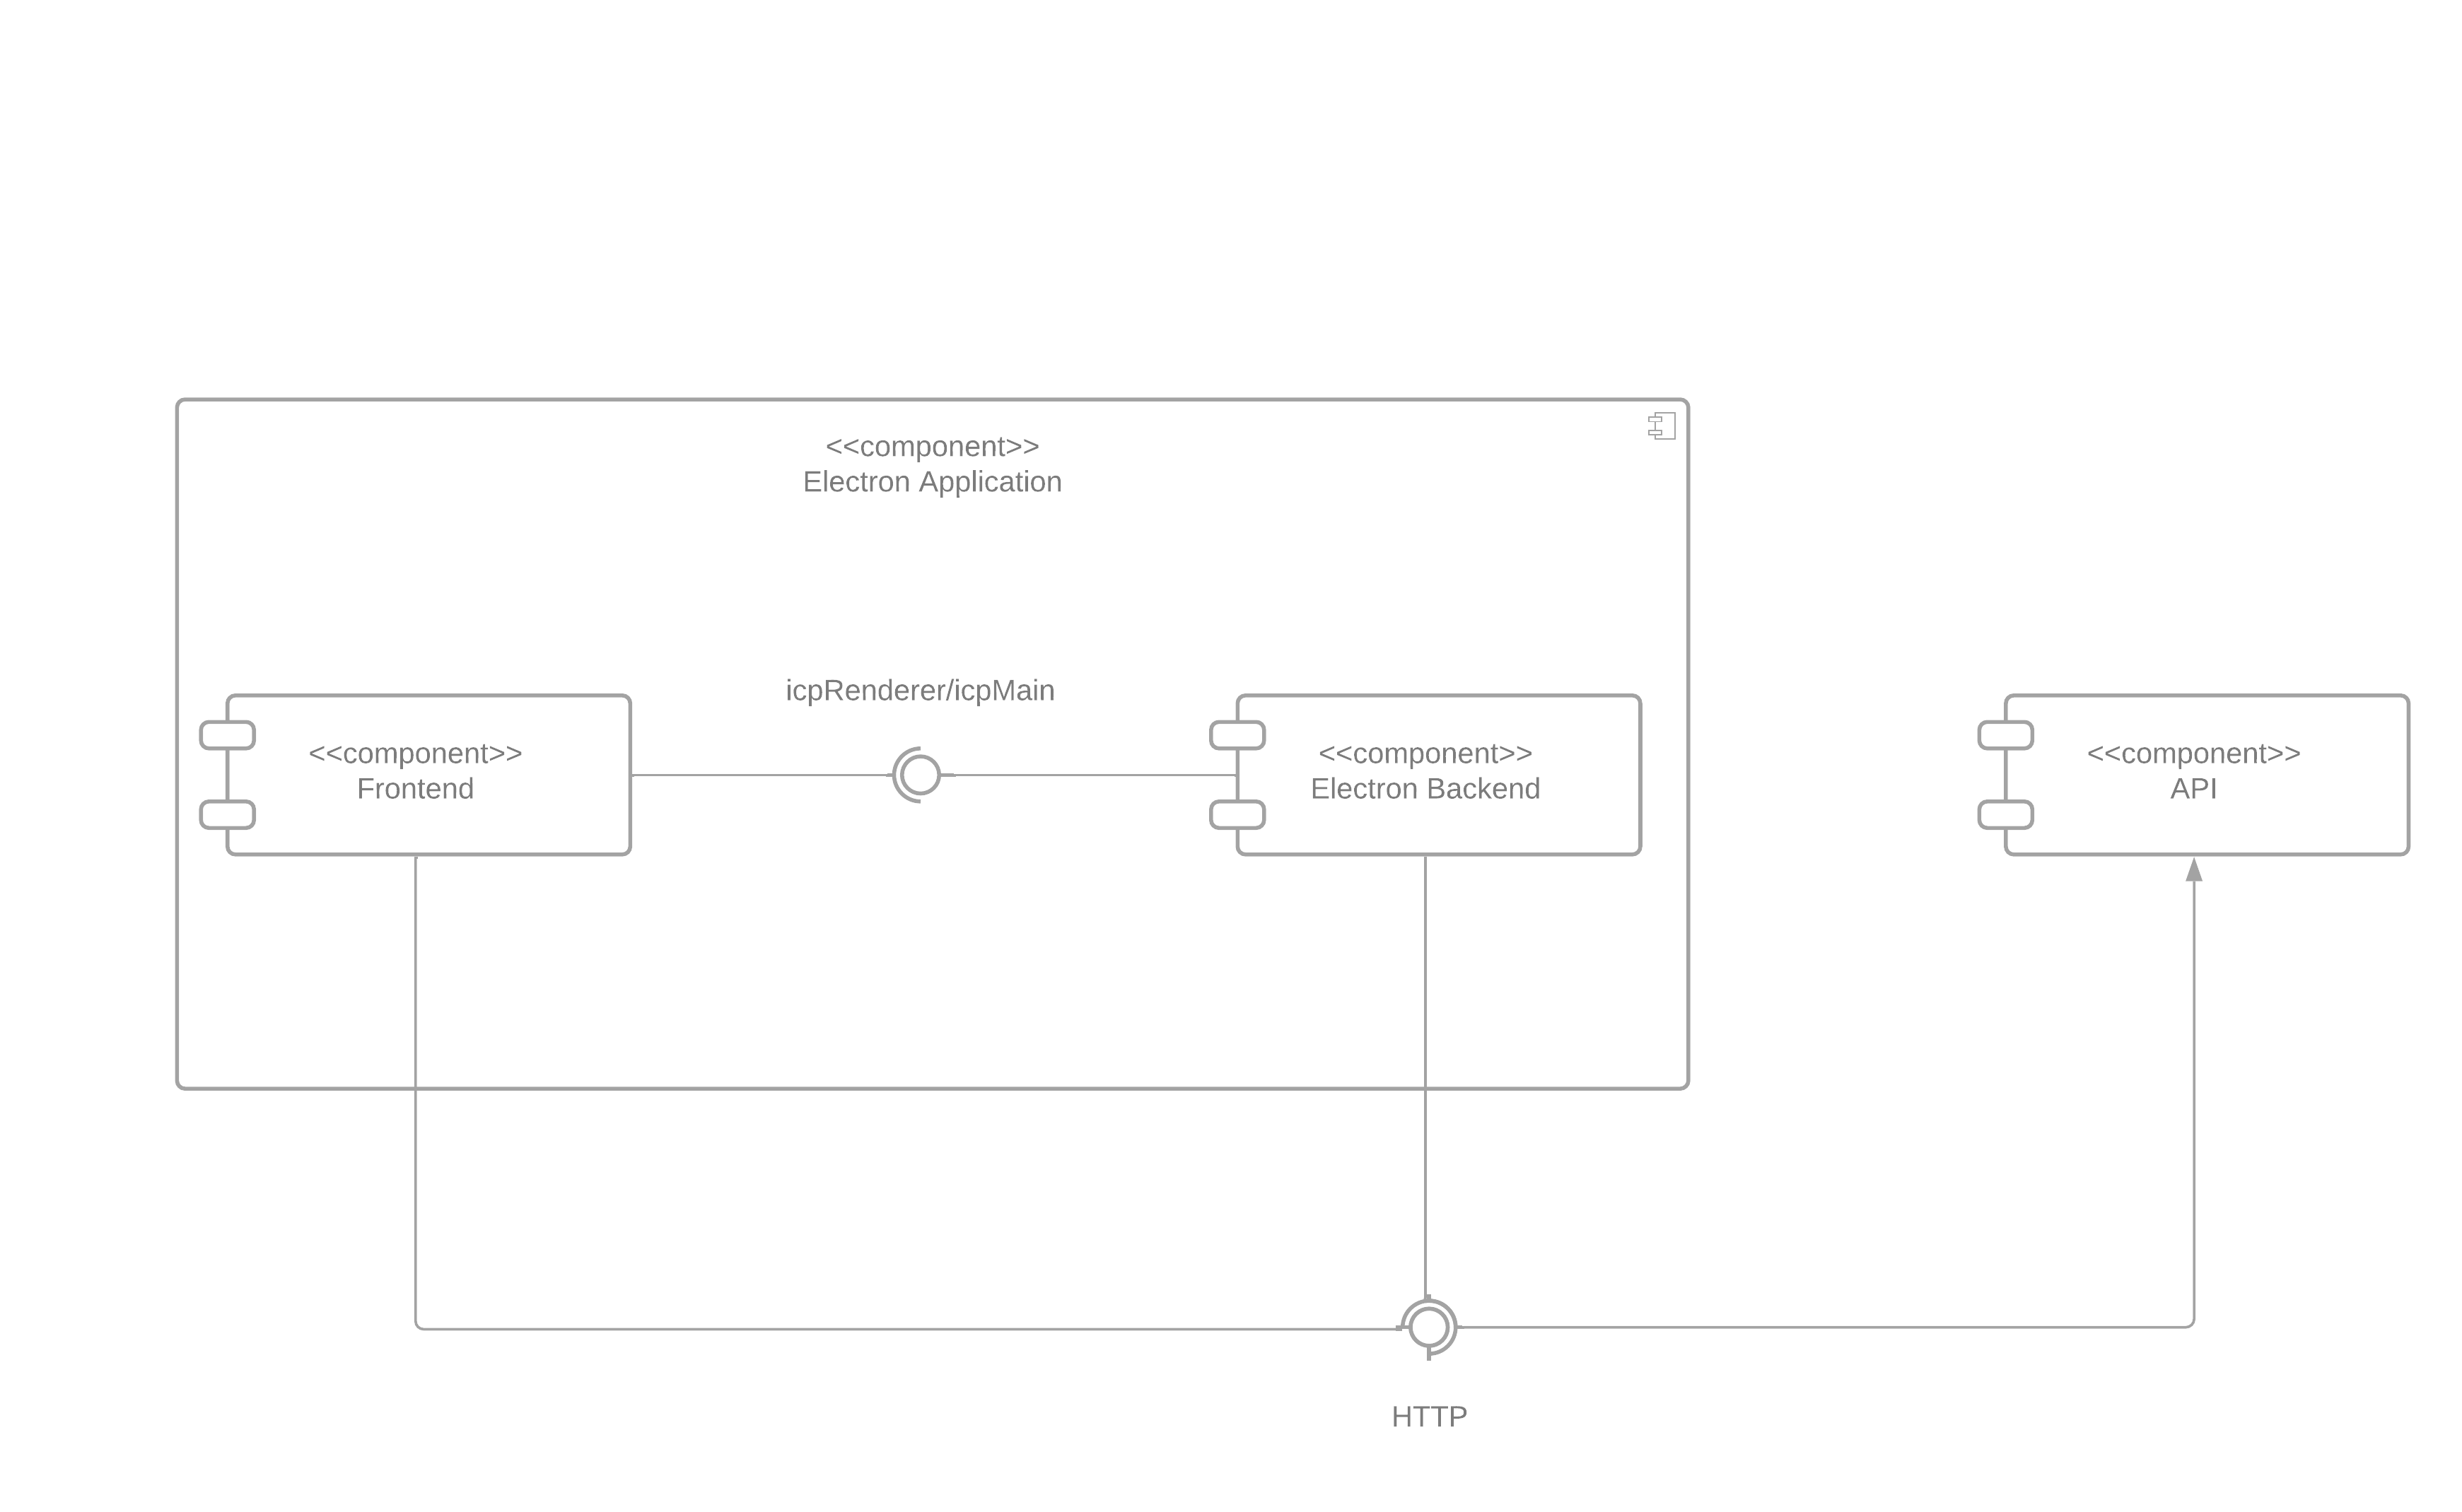
\includegraphics[width=1\textwidth]{pze-component-diagram}
  \caption{A schematic overview of the application components, simplified.}
  \label{fig:pze-component-diagram}
\end{figure}
The above figure shows a simplified overview of the applications's components. 
For the sake of illustration some implementation details have been omitted, such as the details of the database implementation in the 
back-end API.
In essence there are two ways the front-end can communicate with a data source:
Either over HTTP requests with directly the back-end or through the icpMain and icpRenderer processes with the Electron-provided back-end.
The details of this implementation will be discussed in a later chapter. 
To further illustrate the interaction between the application's components, see the following sequence diagram which illustrates
the workflow of creating an entry. 
\begin{figure}[H]
  \centering
  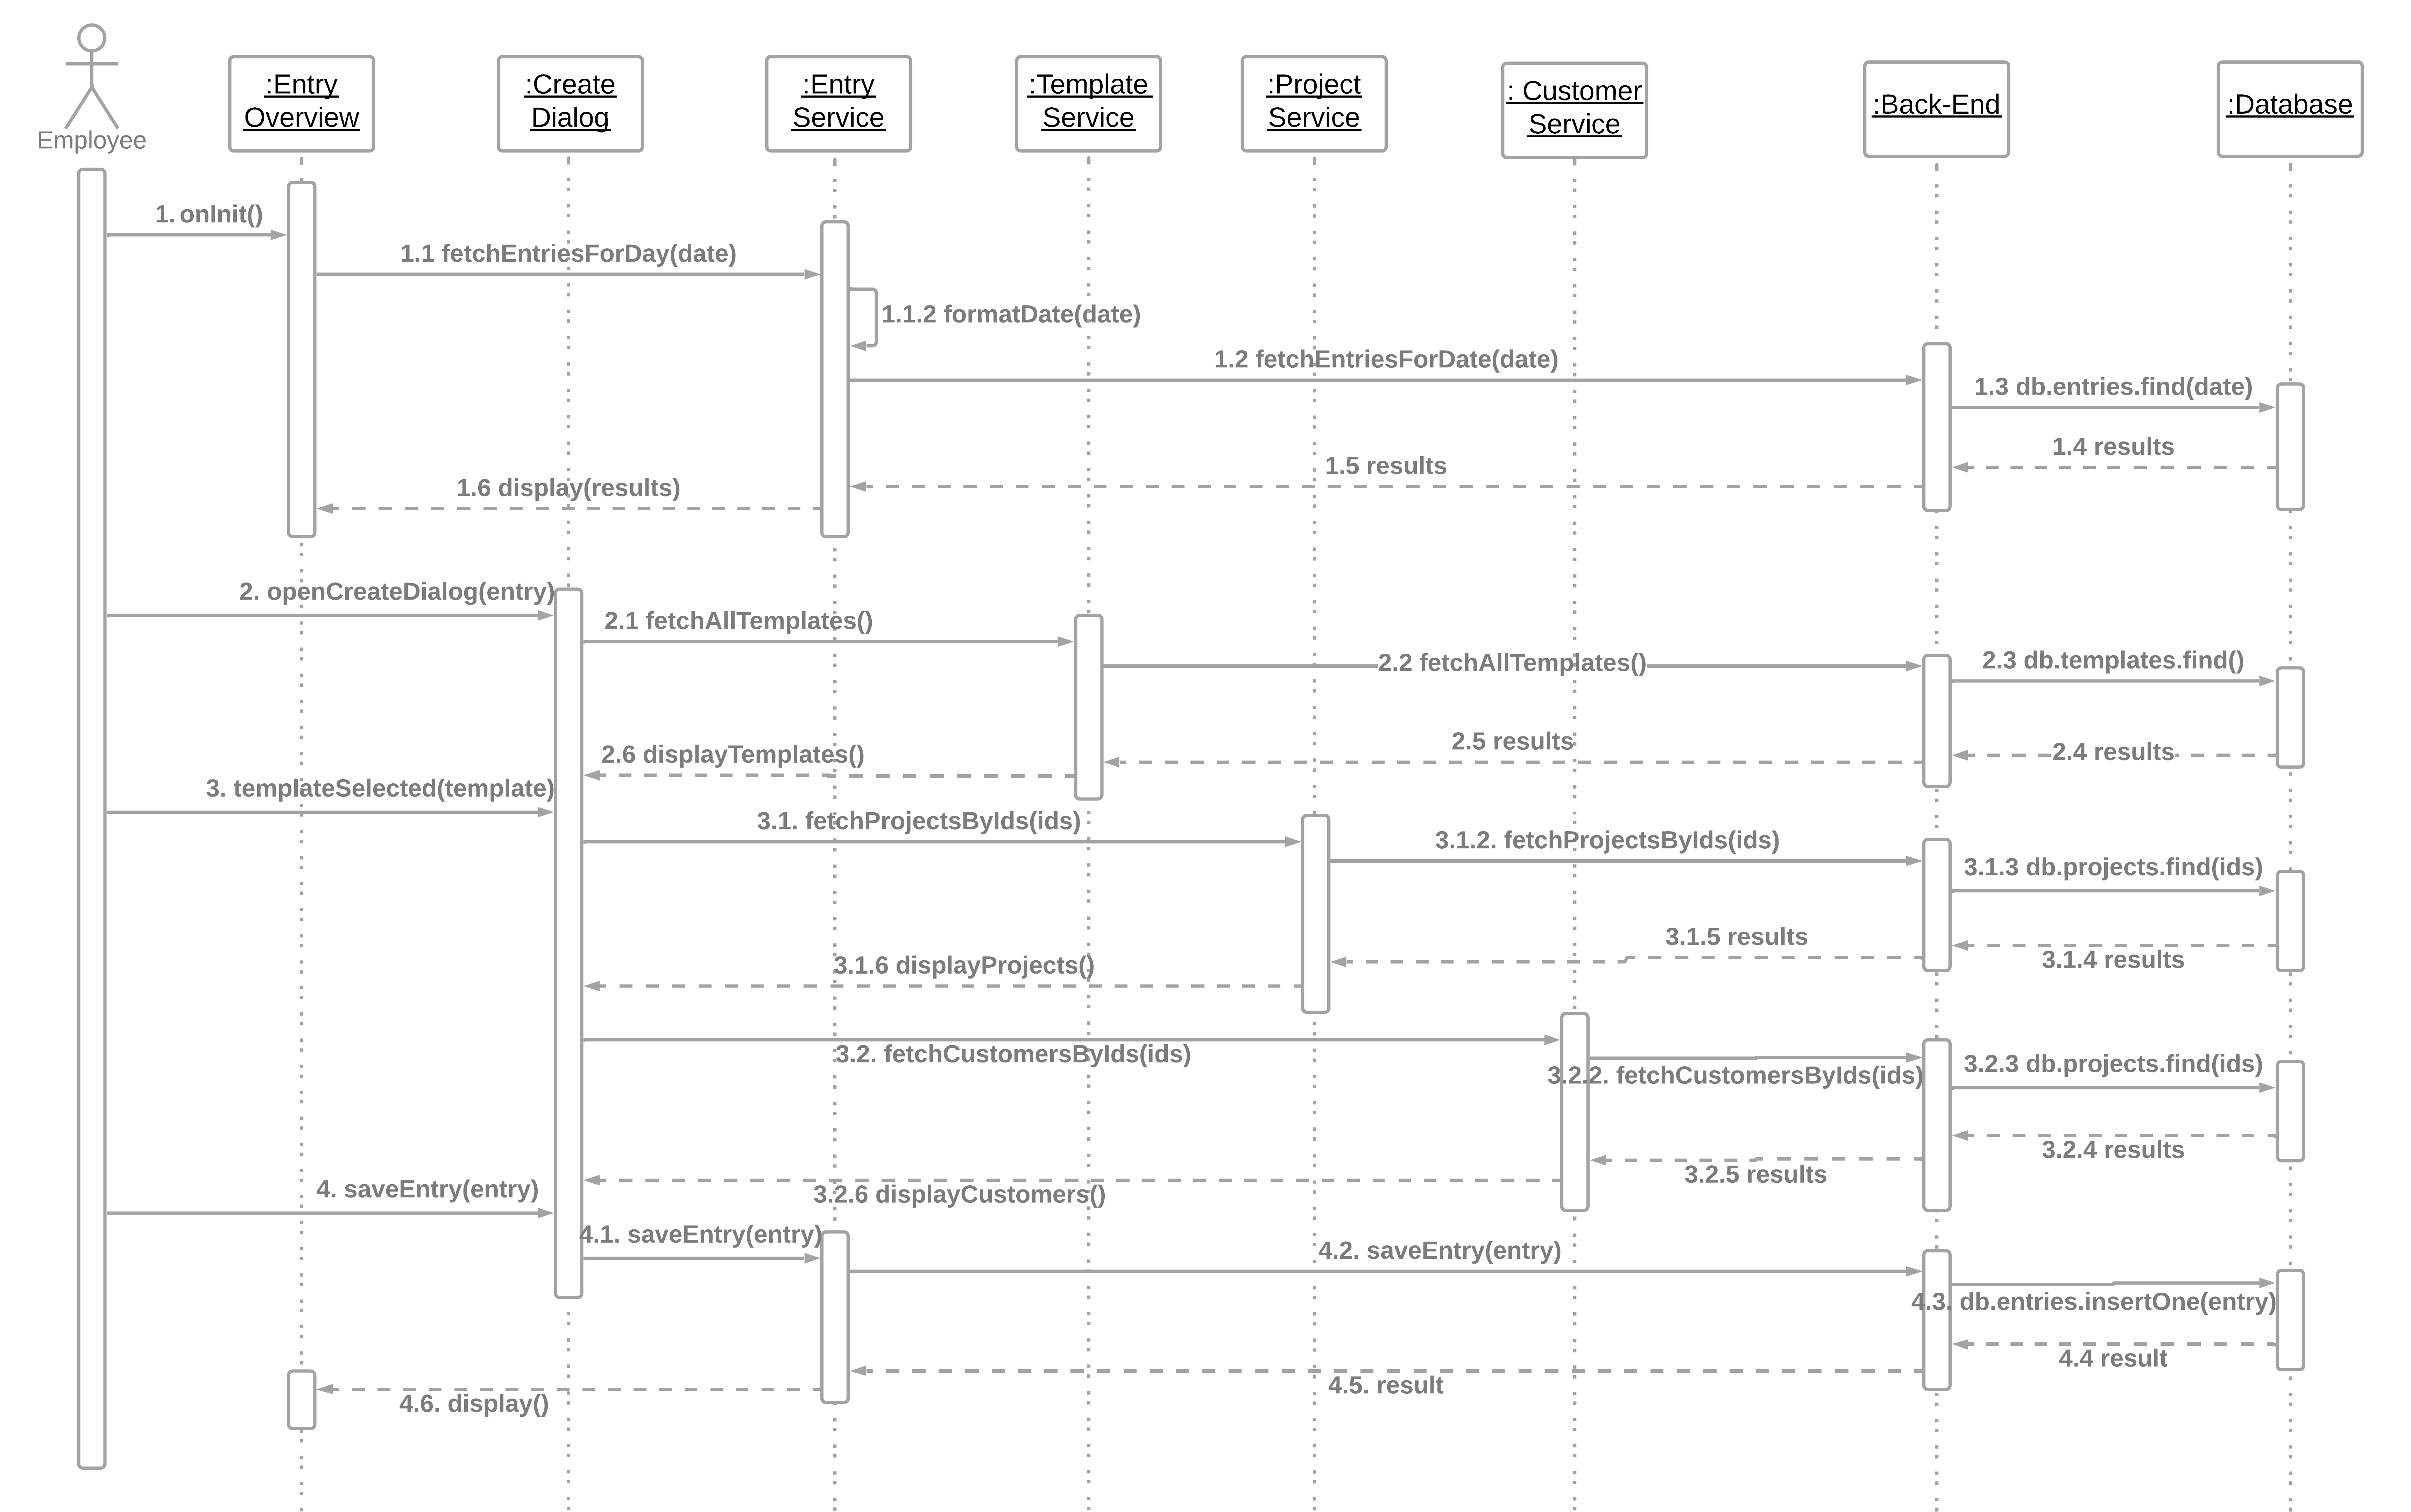
\includegraphics[width=1\textwidth]{pze-sequence-diagram}
  \caption{A sequence diagram of the Create Entry use case.}
  \label{fig:pze-sequence-diagram}
\end{figure}
After the user has started the application they will find themselves on the entry overview which lists all entries for the selected day.
This causes a request to the back-end to fetch all entries for the specified day. 
Once the user opens the create dialog all templates are fetched and displayed to the user to choose from. 
When the user chooses a template the projects and customers defined in the selected template are fetched from the back-end. 
After the user has entered all other necessary data they can save the newly created entry which sends the object to the back-end 
and persists it in the database. 
This is an illustration to show what the workflow behind user creation of an entry looks like and how 
entries, templates, projects and customers all work in accordance.

    \subsection{Developing with Electron}\label{subsec:developing-with-electron}


    \subsubsection{Development Workflow with Electron}\label{subsubsec:dev-workflow}

    \subsubsection{Finished Project}\label{subsubsec:dev-project}


    \section{Analysis}\label{sec:analysis}

    \subsection{Results}\label{subsec:results}

    \subsection{Vaadin as an Alternative to Electron}\label{subsec:vaadin-electron}
    \pagebreak
    \printbibliography
    \pagebreak
    \listoffigures


\end{document}